\typeout{************************************************}
\typeout{Part II Interregnum}
\typeout{************************************************}
%
\begin{partptx}{Interregnum}{}{Interregnum}{}{}{x:part:Interregnum}
	%
	%
	\typeout{************************************************}
	\typeout{Chapter 6 Joseph Fourier: The Man Who Broke Calculus}
	\typeout{************************************************}
	%
	\begin{chapterptx}{Joseph Fourier: The Man Who Broke Calculus}{}{Joseph Fourier: The Man Who Broke Calculus}{}{}{x:chapter:Interegnum}
		%
		%
		\typeout{************************************************}
		\typeout{Section 6.1 Joseph Fourier and His Series}
		\typeout{************************************************}
		%
		\begin{sectionptx}{Joseph Fourier and His Series}{}{Joseph Fourier and His Series}{}{}{g:section:idp92}
			Applying mathematics to physical problems such as heat flow in a solid body drew much attention in the latter part of the 1700's and the early part of the 1800's. One of the people to attack the heat flow problem was%
			\begin{figureptx}{\href{https://mathshistory.st-andrews.ac.uk/Biographies/Fourier/}{Jean Baptiste Joseph Fourier}\protect\footnotemark{}}{g:figure:idp93}{}%
				\index{Fourier, Jean Baptiste Joseph!portrait of}%
				\begin{image}{0.325}{0.35}{0.325}%
					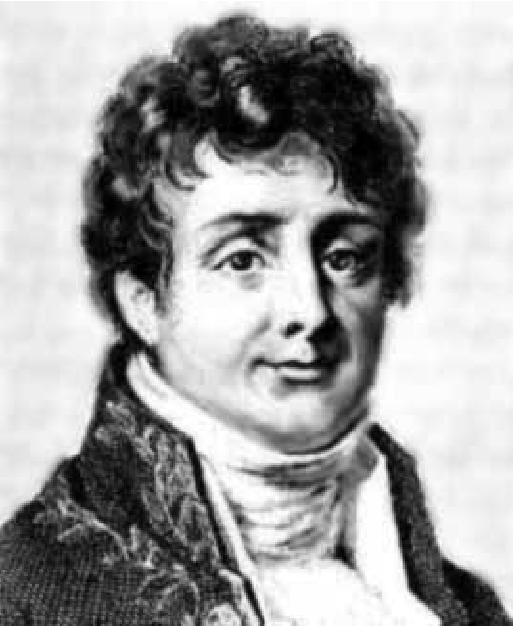
\includegraphics[width=\linewidth]{external/images/Fourier.png}
				\end{image}%
				\tcblower
			\end{figureptx}%
			\footnotetext[13]{\nolinkurl{mathshistory.st-andrews.ac.uk/Biographies/Fourier/}\label{g:fn:idp94}}%
			\index{Fourier, Jean Baptiste Joseph} Jean Baptiste Joseph Fourier.  Fourier submitted a manuscript on the subject, \textit{Sur la propagation de la chaleur} (\emph{On the Propagation of Heat}), to the \textit{Institut National des Sciences et des Arts} in 1807.  These ideas were subsequently published in \textit{La theorie analytique de la chaleur} (\emph{The Analytic Theory of Heat (1822)}).%
			\par
			To examine Fourier's ideas, consider the example of a thin wire of length one, which is perfectly insulated and whose endpoints are held at a fixed temperature of zero. Given an initial temperature distribution in the wire, the problem is to monitor the temperature of the wire at any point \(x\) and at any time \(t\). Specifically, if we let \(u(x,t)\) denote the temperature of the wire at point \(x\in[0,1]\) at time \(t\geq 0\), then it can be shown that \(u\) must satisfy the one-dimensional heat equation \(\rho^2\frac{\partial^2u}{\partial x^2}=\frac{\partial u}{\partial t}\), where \(\rho^2\) is a positive constant known as the thermal diffusivity. If the initial temperature distribution is given by the function \(f(x)\), then the \(u\) we are seeking must satisfy all of the following%
			\begin{equation*}
				\rho^2\frac{\partial^2u}{\partial x^2}=\frac{\partial u}{\partial t}
			\end{equation*}
			%
			\begin{align*}
				u(0,t)\amp =u(1,t)=0,\ \ \forall\,t\geq 0\\
				u(x,0)\amp =f(x),\ \ \forall\,x\in[\,0,1]\text{.}
			\end{align*}
			%
			\par
			To solve this, Fourier employed what is now referred to as Fourier's method of separation of variables. Specifically, Fourier looked for solutions of the form \(u(x,t)=X(x)T(t)\); that is, solutions where the \(x\)-part can be separated from the \(t\)-part. Assuming that \(u\) has this form, we get \(\frac{\partial^2u}{\partial x^2}=X^{\prime\prime}T\) and \(\frac{\partial u}{\partial t}=X\,T^{\prime}\). Substituting these into the differential equation \(\rho^2\frac{\partial^2u}{\partial x^2}=\frac{\partial u}{\partial t}\), we obtain%
			\begin{equation*}
				\rho^2X^{\prime\prime}T=X T^\prime\text{  or  } \frac{X^{\prime\prime}}{X}=\frac{T^\prime}{\rho^2T}\text{.}
			\end{equation*}
			%
			\par
			Since the left-hand side involves no \(t\)'s and the right-hand side involves no \(x\)'s, both sides must equal a constant \(k\). Thus we have%
			\begin{equation*}
				X^{\prime\prime}=k X\text{ and } T^\prime=\rho^2k T\text{.}
			\end{equation*}
			%
			\begin{problem}{}{x:problem:prob_HarmonicMotion}%
				\index{Heat Equation, the}\index{Heat Equation, the!parameter \(k\) must be less than zero} Show that \(T=Ce^{\rho^2kt}\) satisfies the equation \(T^\prime=\rho^2k T\), where \(C\), and \(\rho\) are arbitrary constants. Use the physics of the problem to show that if \(u\) is not constantly zero, then \(k\lt 0\).%
				\par\smallskip%
				\noindent\textbf{\blocktitlefont Hint}.\hypertarget{g:hint:idp95}{}\quad{}Consider \(\lim_{t\rightarrow\infty}u(x,t)\).%
			\end{problem}
			Using the result from \hyperref[x:problem:prob_HarmonicMotion]{problem~{\xreffont\ref{x:problem:prob_HarmonicMotion}}} that \(k\lt 0\), we will let \(k=-p^2\).%
			\begin{problem}{}{g:problem:idp96}%
				\index{Heat Equation, the}\index{Heat Equation, the!solving for \(\xi(x)\)} Show that \(X=A\sin\left(px\right)+B\cos\left(px\right)\) satisfies the equation \(X\,''=-p^2X\), where \(A\) and \(B\) are arbitrary constants. Use the boundary conditions \(u(0,t)=u(1,t)=0\), \(\forall\,t\geq 0\) to show that \(B=0\) and \(A\sin p=0\). Conclude that if \(u\) is not constantly zero, then \(p=n\pi\), where \(n\) is any integer.%
			\end{problem}
			\begin{problem}{}{g:problem:idp97}%
				\index{Heat Equation, the!fundamental solutions of}%
				\par
				Show that if \(u_1\) and \(u_2\) satisfy the equations \(\rho^2\frac{\partial^2u}{\partial x^2}=\frac{\partial
					u}{\partial t}\) and \(u(0,t)=u(1,t)=0, \forall\,t\geq
				0\) then \(u=A_1u_1+A_2u_2\) satisfy these as well, where \(A_1\) and \(A_2\) are arbitrary constants.%
			\end{problem}
			\index{Fourier, Jean Baptiste Joseph} Putting all of these results together, Fourier surmised that the general solution to%
			\begin{equation*}
				\rho^2\frac{\partial^2u}{\partial x^2}=\frac{\partial u}{\partial t} u(0,t)=u(1,t)=0, \,\forall\,t\geq 0
			\end{equation*}
			could be expressed as the series%
			\begin{equation*}
				u(x,t)=\sum_{n=1}^\infty A_ne^{-(\rho n\pi)^2t}\sin\left(n\pi x\right)\text{.}
			\end{equation*}
			%
			\par
			All that is left is to have \(u\) satisfy the initial condition \(u(x,0)=f(x)\), \(\forall\,x\in[\,0,1]\). That is, we need to find coefficients \(A_n\), such that%
			\begin{equation*}
				f(x)=u(x,0)=\sum_{n=1}^\infty A_n\sin\left(n\pi x\right)\text{.}
			\end{equation*}
			%
			\par
			The idea of representing a function as a series of sine waves was proposed by Daniel Bernoulli in 1753 while examining the problem of modeling a vibrating string. Unfortunately for Bernoulli, he didn't know how to compute the coefficients in such a series representation. What distinguished Fourier was that he developed a technique to compute these coefficients. The key is the result of the following problem.%
			\begin{problem}{}{x:problem:prob_SinOrthogonality}%
				\index{\(\sin x\)!orthogonality of}\index{orthogonality!of \(\sin nx\)} Let \(n\) and \(m\) be positive integers. Show%
				\begin{equation*}
					\int_{x=0}^1\sin\left(n\pi x\right)\sin\left(m\pi x\right)\dx{ x}= \left\{\begin{matrix}0\amp \text{ if } n\neq m\\ \frac{1}{2}\amp \text{ if } n=m \end{matrix} \right.. {}
				\end{equation*}
				%
			\end{problem}
			Armed with the result from \hyperref[x:problem:prob_SinOrthogonality]{Problem~{\xreffont\ref{x:problem:prob_SinOrthogonality}}}, \index{Fourier, Jean Baptiste Joseph} Fourier could compute the coefficients \(A_n\) in the series representation \(f(x)=\sum_{n=1}^\infty A_n \sin\left(n\pi x\right)\) in the following manner. Since we are trying to find \(A_n\) for a particular (albeit general) \(n\), we will temporarily change the index in the summation from \(n\) to \(j\). With this in mind, consider%
			\begin{align*}
				\int_{x=0}^1f(x)\sin\left(n\pi x\right)\dx{ x} \amp =\int_{x=0}^1\left(\sum_{j=1}^\infty A_j\text{ sin } \left(j\pi x\right)\right)\sin\left(n\pi x\right)\dx{ x}\\
				\amp =\sum_{j=1}^\infty A_j\int_{x=0}^1\sin\left(j\pi x\right)\sin\left(n\pi x\right)\dx{ x}\\
				\amp =A_n\cdot\frac{1}{2}
			\end{align*}
			%
			\par
			This leads to the formula \(A_n=2\int_{x=0}^1f(x)\sin\left(n\pi x\right)d x\).%
			\par
			The above series \(f(x)=\sum_{n=1}^\infty A_n\sin\left(n\pi x\right)\) with \(A_n=2\int_{x=0}^1f(x)\sin\left(n\pi x\right)\dx{ x}\) is called the \emph{Fourier (sine) series of \(\boldsymbol{f}\)}.%
			\begin{example}{}{g:example:idp98}%
				Let's apply this to the following function, \(f(x)=\frac{1}{2}-\abs{x-\frac{1}{2}}\), whose graph of this function is seen below.%
				\begin{image}{0.125}{0.75}{0.125}%
					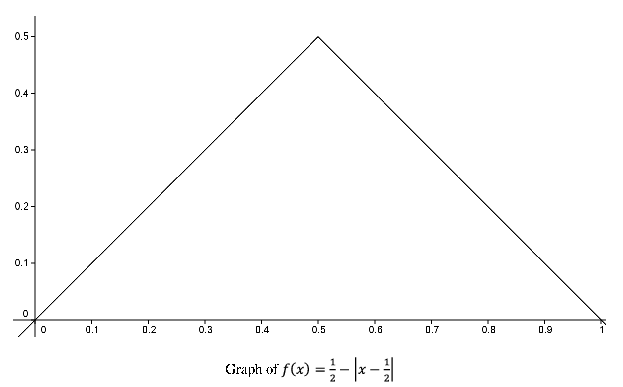
\includegraphics[width=\linewidth]{external/images/FourierEx1.png}
				\end{image}%
			\end{example}
			\begin{problem}{}{g:problem:idp99}%
				\index{Fourier Series!sine series of an odd function} Let \(n\) be a positive integer. Show that if%
				\begin{equation*}
					f(x)=\frac{1}{2}-\abs{x-\frac{1}{2}}
				\end{equation*}
				then%
				\begin{equation*}
					\int_{x=0}^1f(x)\sin\left(n\pi x\right)d x = \frac{2}{\left(n\pi\right)^2}\sin\left(\frac{n\pi}{2}\right)
				\end{equation*}
				and show that the Fourier sine series of \(f\) is given by%
				\begin{equation*}
					f(x)=\sum_{n=1}^\infty\frac{4}{\left(n\pi\right)^2}\sin\left(\frac{n\pi}{2} \right)\sin\left(n\pi x\right)=\frac{4}{\pi^2}\sum_{k=0}^\infty\frac{\left(-1\right)^k}{\left(2k+1\right)^2}\sin\left(\left(2k+1\right)\pi x\right).{}
				\end{equation*}
				%
			\end{problem}
			To check if this series really does, in fact, represent \(f\) on \([0,1]\), let%
			\begin{equation*}
				S_N(x)=\frac{4}{\pi^2}\sum_{k=0}^N\frac{\left(-1\right)^k}{\left(2k+1\right)^2} \sin\left(\left(2k+1\right)\pi x\right)
			\end{equation*}
			be the \(N^{th}\) partial sum of the series and use the graphing tool below to view the graph of \(S_N(x)\) for several values of \(N\).%
			\par
			That is, \(S_N\) denotes the \(N^{th}\) partial sum of the series. We will graph \(S_N\) for \(N=1,\,2,\,5,\,50\).%
			\par
			%
			\begin{figureptx}{}{g:figure:idp100}{}%
				\centering
				\begin{image}{0}{1}{0}%
					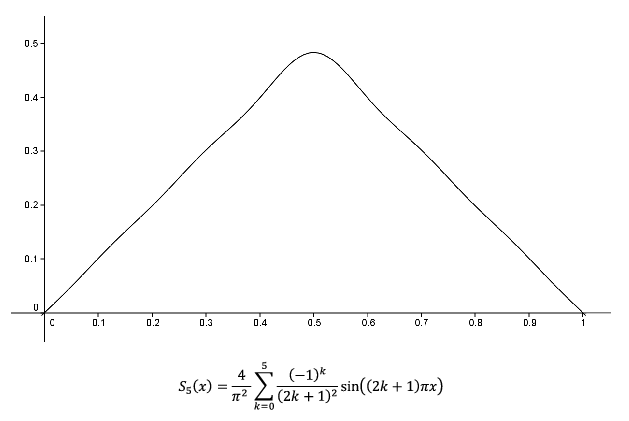
\includegraphics[width=\linewidth]{external/images/FourierEx4.png}
				\end{image}%
				\tcblower
			\end{figureptx}%
			As you can see, it appears that as we add more terms to the partial sum, \(S_N\), it looks more and more like the original function \(f(x)=\frac{1}{2}-\abs{x-\frac{1}{2}}\). This would lead us to believe that the series converges to the function and that%
			\begin{equation}
				f(x)=\frac{4}{\pi^2}\sum_{k=0}^\infty\frac{\left(-1\right)^k}{\left(2k+1\right)^2}\sin\left(\left(2k+1\right)\pi x\right)\text{.}\label{x:men:PDE_sol}
			\end{equation}
			is a valid representation of \(f\) as a Fourier series.%
			\par
			Recall, that when we represented a function as a power series, we freely differentiated and integrated the series term by term as though it was a polynomial. Let's do the same with this Fourier series.%
			\par
			To start, notice that the derivative of%
			\begin{equation*}
				f(x)=\frac{1}{2}-\abs{x-\frac{1}{2}}
			\end{equation*}
			is given by%
			\begin{equation*}
				f^\prime(x) = \begin{cases}1\amp \text{ if } \,\text{ } 0\leq x\lt \frac{1}{2}\\ -1\amp \text{ if } \,\frac{1}{2}\lt x\leq 1 \end{cases} \text{.}
			\end{equation*}
			%
			\par
			This derivative does not exist at \(x=\frac{1}{2}\) and its graph is given by%
			\begin{image}{0.125}{0.75}{0.125}%
				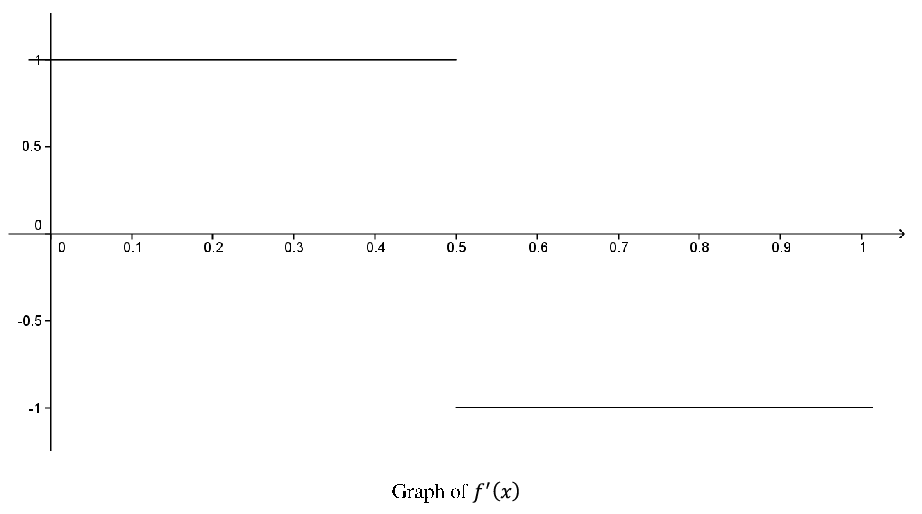
\includegraphics[width=\linewidth]{external/images/Ch2fig1.png}
			\end{image}%
			If we differentiate the Fourier series term-by-term, we obtain%
			\begin{equation*}
				\frac{4}{\pi}\sum_{k=0}^\infty\frac{\left(-1\right)^k}{\left(2k+1\right)} \cos\left(\left(2k+1\right)\pi x\right)\text{.}
			\end{equation*}
			%
			\par
			Again, if we let \(C_N(x)=\frac{4}{\pi}\sum_{k=0}^N\frac{\left(-1\right)^k}{\left(2k+1\right)} \cos\left(\left(2k+1\right)\pi x\right)\) be the \(N^{th}\) partial sum of this Fourier cosine series and plot \(C_N(x)\) for \(N=1,2,5,50\), we obtain%
			\begin{figureptx}{}{g:figure:idp101}{}%
				\centering
				\begin{image}{0}{1}{0}%
					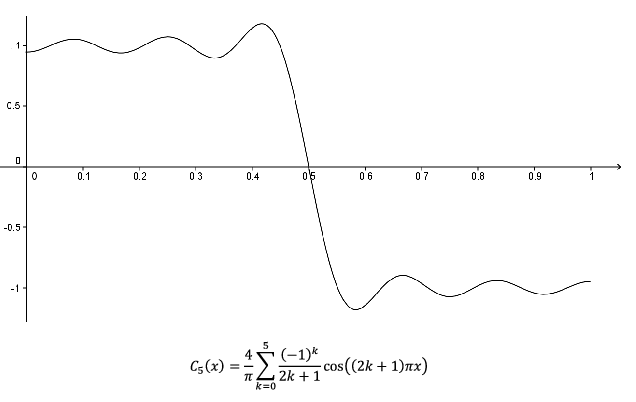
\includegraphics[width=\linewidth]{external/images/FourierEx8.png}
				\end{image}%
				\tcblower
			\end{figureptx}%
			In fact, if we were to graph the series \(\frac{4}{\pi}\sum_{k=0}^\infty\frac{\left(-1\right)^k}{\left(2k+1\right)}\) cos\(\left(\left(2k+1\right)\pi x\right)\), we would obtain%
			\begin{sidebyside}{1}{0.05}{0.05}{0}%
				\begin{sbspanel}{0.9}[center]%
					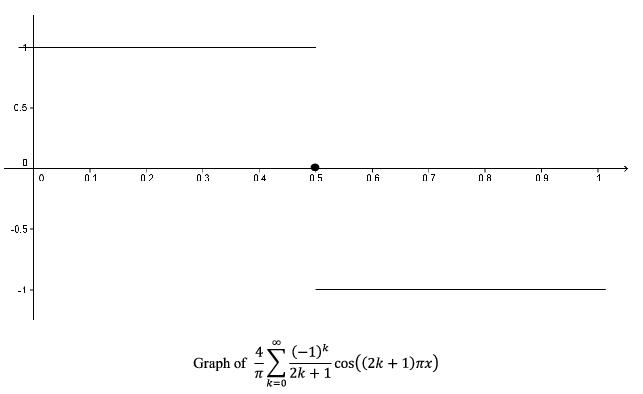
\includegraphics[width=\linewidth]{external/images/FourierEx10.png}
				\end{sbspanel}%
			\end{sidebyside}%
			\par
			Notice that this agrees with the graph of \(f^\prime\), except that \(f^\prime\) didn't exist at \(x=\frac{1}{2}\), and this series takes on the value \(0\) at \(x=\frac{1}{2}\). Notice also, that every partial sum of this series is continuous, since it is a finite combination of continuous cosine functions. This agrees with what you learned in calculus, the (finite) sum of continuous functions is always continuous. In the 1700's, this was also assumed to be true for infinite series, because every time a power series converged to a function, that function happened to be continuous. This never failed for power series, so this example was a bit disconcerting as it is an example of the sum of \emph{infinitely many} continuous functions which is, in this case, discontinuous. Was it possible that there was some power series which converged to a function which was not continuous? Even if there wasn't, what was the difference between power series and this Fourier series?%
			\par
			Even more disconcerting is what happens if we try differentiating the series%
			\begin{equation*}
				\frac{4}{\pi}\sum_{k=0}^\infty\frac{\left(-1\right)^k}{\left(2k+1\right)} \cos\left(\left(2k+1\right)\pi x\right)
			\end{equation*}
			term-by-term. Given the above graph of this series, the derivative of it should be constantly 0, except at \(x=\frac{1}{2}\), where the derivative wouldn't exist. Using the old adage that the derivative of a sum is the sum of the derivatives, we differentiate this series term-by-term to obtain the series%
			\begin{equation*}
				4\sum_{k=0}^\infty\left(-1\right)^{k+1}\sin\left(\left(2k+1\right)\pi x\right)\text{.}
			\end{equation*}
			%
			\par
			If we sum the first forty terms of this series, we get \begin{figureptx}{}{g:figure:idp102}{}%
				\centering
				\begin{image}{0}{1}{0}%
					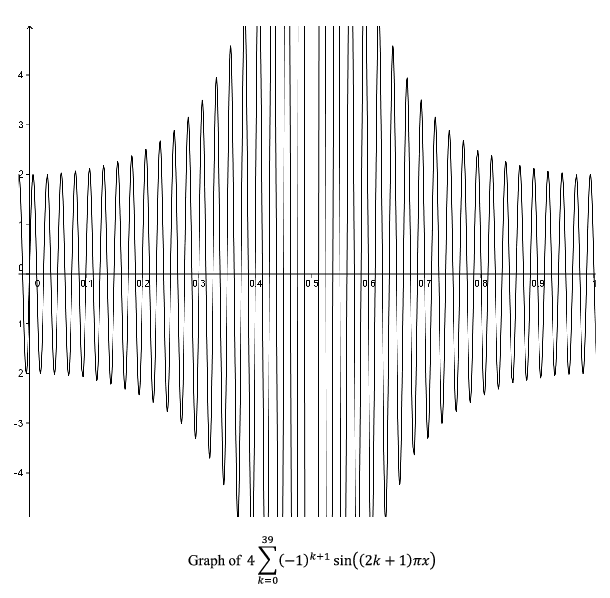
\includegraphics[width=\linewidth]{external/images/FourierEx11.png}
				\end{image}%
				\tcblower
			\end{figureptx}%
			%
			\par
			We knew that there might be a problem at \(x=\frac{1}{2}\) but this is crazy! The series seems to not be converging to zero at all!%
			\begin{problem}{}{x:problem:prob_FourierDiverge}%
				\index{Fourier Series}\index{Fourier Series!divergent Fourier series example} Show that when \(x=\frac{1}{4}\)%
				\begin{equation*}
					4\sum_{k=0}^\infty\left(-1\right)^{k+1} \sin\left(\left(2k+1\right)\pi x\right)=4\left(-\frac{1}{\sqrt{2}}+\frac{1}{\sqrt{2}}+\frac{1}{\sqrt{2}}- \frac{1}{\sqrt{2}}-\frac{1}{\sqrt{2}}+\cdots\right)\text{.}
				\end{equation*}
				%
			\end{problem}
			\hyperref[x:problem:prob_FourierDiverge]{Problem~{\xreffont\ref{x:problem:prob_FourierDiverge}}} shows that when we differentiate the series%
			\begin{equation*}
				\frac{4}{\pi}\sum_{k=0}^\infty\frac{\left(-1\right)^k}{\left(2k+1\right)} \cos\left(\left(2k+1\right)\pi x\right)
			\end{equation*}
			term by term, this differentiated series doesn't converge to anything at \(x=\frac{1}{4}\), let alone converge to zero. In this case, the old calculus rule that the derivative of a sum is the sum of the derivatives does not apply for this infinite sum, though it did apply before. As if the continuity issue wasn't bad enough before, this was even worse. Power series were routinely differentiated and integrated term-by-term. This was part of their appeal. They were treated like ``infinite polynomials.'' Either there is some power series lurking that refuses to behave nicely, or there is some property that power series have that not all Fourier series have.%
			\par
			Could it be that everything we did in \hyperref[x:chapter:PowerSeriesQuestions]{Chapter~{\xreffont\ref{x:chapter:PowerSeriesQuestions}}} was bogus?%
			\par
			Fortunately, the answer to that question is no. Power series are generally much more well-behaved than Fourier series. Whenever a power series converges, the function it converges to will be continuous. As long as one stays inside the interval of convergence, power series can be differentiated and integrated term-by-term. Power series have something going for them that your average Fourier series does not. (We need to develop the machinery to know what that something is.) None of this is any more obvious to us than it was to mathematicians at the beginning of the nineteenth century. What they did know was that relying on intuition was perilous and rigorous formulations were needed to either justify or dismiss these intuitions. In some sense, the nineteenth century was the ``morning after'' the mathematical party that went on throughout the eighteenth century.%
			\begin{problem}{}{x:problem:prob_Fourier_Series-orthogonality}%
				\index{\(\cos (nx)\)!orthogonality of}\index{orthogonality!of \(\cos nx\)} Let \(n\) and \(m\) be positive integers. Show%
				\begin{equation*}
					\int_{x=0}^1\cos\left(n\pi x\right)\cos\left(m\pi x\right)\dx{ x}=\left\{ \begin{matrix}0\amp \text{ if } n\neq m\\ \frac{1}{2}\amp \text{ if } n=m \end{matrix} \right.\text{.}
				\end{equation*}
				%
			\end{problem}
			\begin{problem}{}{x:problem:prob_fouriercoef}%
				\index{Fourier Series!computing the coefficients} Use the result of \hyperref[x:problem:prob_Fourier_Series-orthogonality]{Problem~{\xreffont\ref{x:problem:prob_Fourier_Series-orthogonality}}} to show that if%
				\begin{equation*}
					f(x)=\sum_{n=1}^\infty B_n\cos\left(n\pi x\right)
				\end{equation*}
				on \([0,1]\), then%
				\begin{equation*}
					B_m=2\int_{x=0}^1f(x)\cos\left(m\pi x\right)\dx{ x}.{}
				\end{equation*}
				%
			\end{problem}
			\begin{problem}{}{g:problem:idp103}%
				\index{Fourier Series!cosine series!the Fourier cosine series of \(f(x)=x-\frac{1}{2}\)} Apply the result of \hyperref[x:problem:prob_fouriercoef]{Problem~{\xreffont\ref{x:problem:prob_fouriercoef}}} to show that the Fourier cosine series of \(f(x)=x-\frac{1}{2}\) on \([0,1]\) is given by%
				\begin{equation*}
					\frac{-4}{\pi^2}\sum_{k=0}^\infty\frac{1}{\left(2k+1\right)^2}\cos \left((2k+1)\pi x\right)\text{.}
				\end{equation*}
				%
				\par
				Let \(C(x,N)=\frac{-4}{\pi^2}\sum_{k=0}^N\frac{1}{\left(2k+1\right)^2}\cos \left((2k+1)\pi x\right)\) and plot \(C(x,N)\) for \(N=1,2,5,50\) \(x\in[\,0,1]\). How does this compare to the function \(f(x)=x-\frac{1}{2}\) on \([\,0,1]\)? What if you plot it for \(x\in[\,0,2]?\)%
			\end{problem}
			\begin{problem}{}{g:problem:idp104}%
				\begin{enumerate}[font=\bfseries,label=(\alph*),ref=\alph*]
					\item{}Differentiate the series%
					\begin{equation*}
						\frac{-4}{\pi^2}\sum_{k=0}^\infty\frac{1}{\left(2k+1\right)^2}\cos \left((2k+1)\pi x\right)
					\end{equation*}
					term by term and plot various partial sums for that series on \([\,0,1]\). How does this compare to the derivative of \(f(x)=x-\frac{1}{2}\) on that interval?%
					\item{}Differentiate the series you obtained in part a and plot various partial sums of that on \([\,0,1]\). How does this compare to the second derivative of \(f(x)=x-\frac{1}{2}\) on that interval?%
				\end{enumerate}
			\end{problem}
		\end{sectionptx}
	\end{chapterptx}
\end{partptx}
%
%